\documentclass[11pt]{article}
\usepackage[a4paper,margin=1in]{geometry}
\usepackage{hyperref}
\usepackage{enumitem}
\usepackage{parskip}
\usepackage{graphicx}
\usepackage{booktabs}

\hypersetup{colorlinks=true,urlcolor=blue,linkcolor=black}
\setlist{nosep,leftmargin=*}

\title{\vspace{-2em}CS5013 Design Document\\[0.3em]
\large Exchange Student Guide \& Community Platform}
\author{Mikhail Novikov, Roll no.\ GE26Z858 \and Abdirakhim Ismailov, Roll no.\ GE26Z860}
\date{11 September 2026}

\begin{document}
\sloppy
\maketitle

\vspace{-1em}
\noindent\rule{\textwidth}{0.4pt}

\noindent Repository: \url{https://github.com/rikire/Exchange-Student-Guide-Platform}. Every claim
below names the file it comes from, so anything here can be checked against the code rather than
taken on trust.

\vspace{0.4em}
\noindent\begin{tabular}{@{}lll@{}}
\toprule
\textbf{What the rubric asks} & \textbf{Section} & \textbf{Evidence in the repository} \\
\midrule
Modules and interfaces & \S1 & \texttt{docs/architecture/}, \texttt{ModularityTest} \\
One test per module & \S2 & \texttt{docs/roadmap/01-requirements-design.md} \\
Milestones revised after feedback & \S3 & \texttt{docs/course/scoping-feedback.md} \\
Risks and plan B & \S4 & \texttt{docs/roadmap/}, this document \\
\bottomrule
\end{tabular}

\noindent\rule{\textwidth}{0.4pt}

\section{The slice boundary is enforced by a test}

The application is a vertical-slice monolith on Spring Modulith. A slice is one feature with its own
controller, service, domain logic, repository, templates and tests. We weighed a layered build
against it and rejected that, in ADR-0002. Ten slices, plus a \texttt{shared} module holding the JPA
entities and migrations, the page layout and the security configuration.

\begin{figure}[h]
\centering
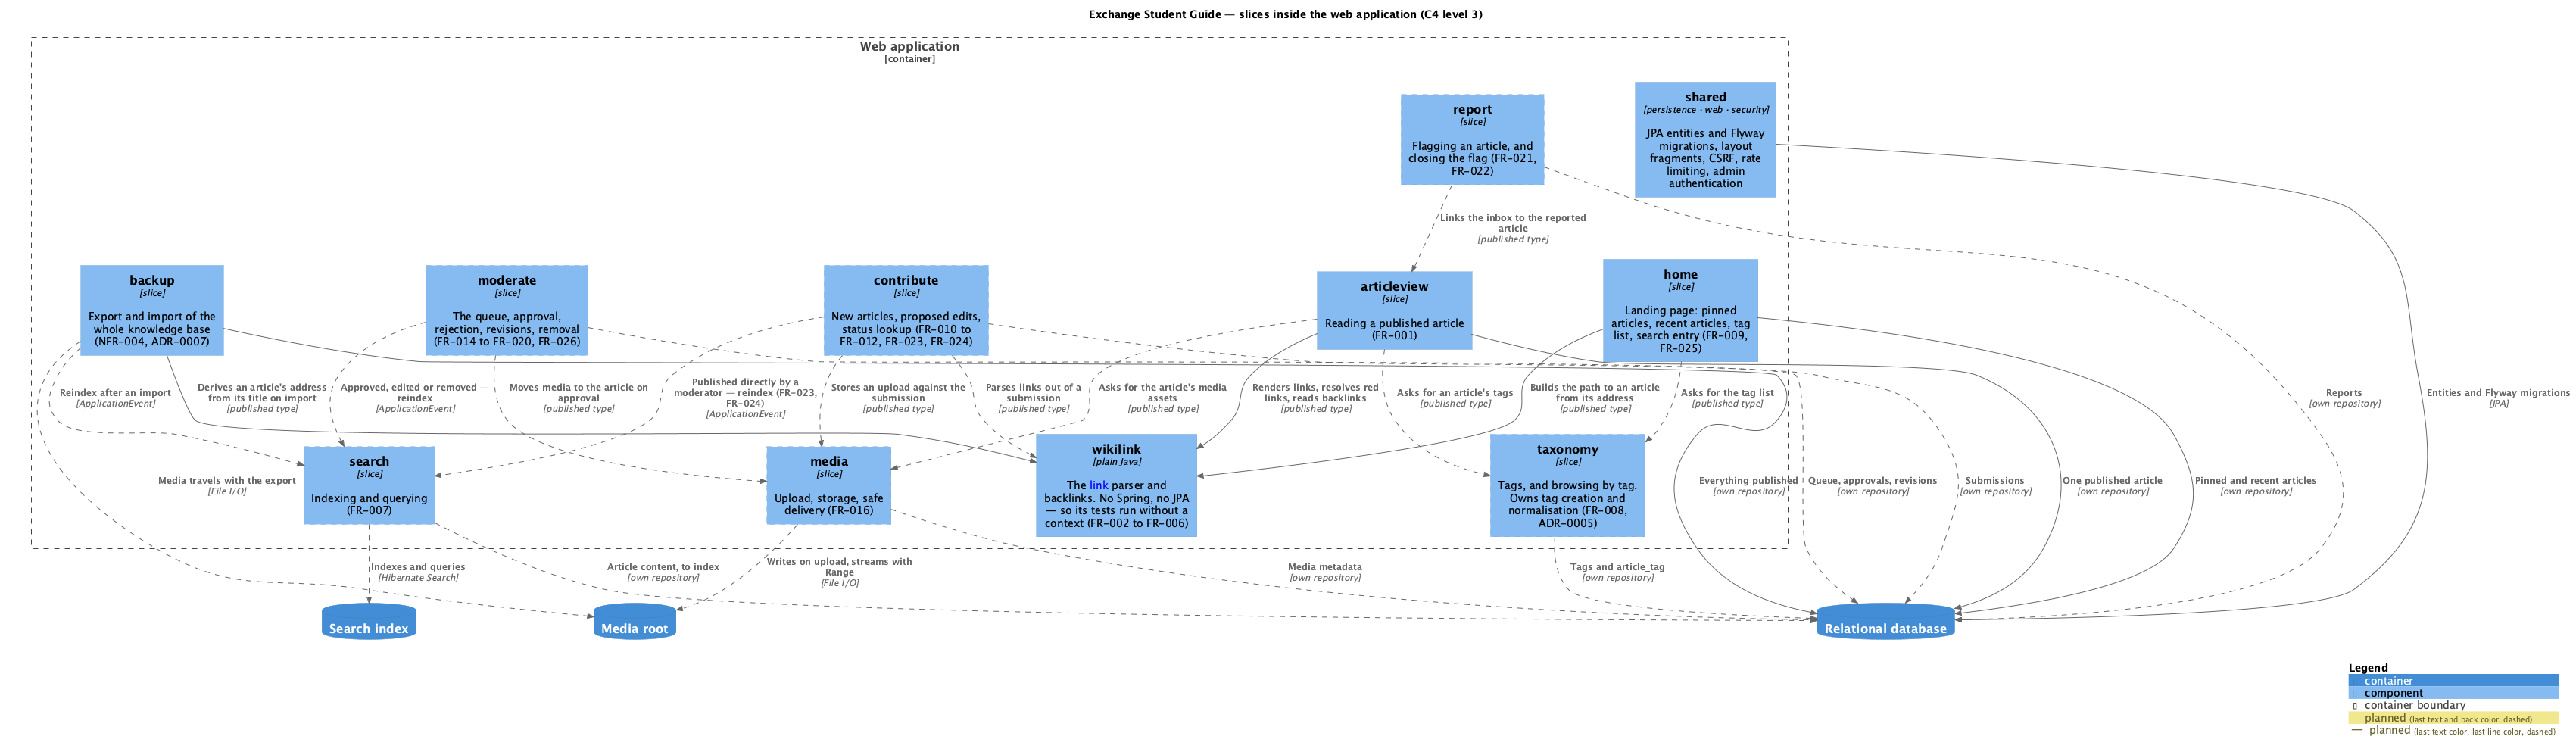
\includegraphics[width=\textwidth]{../diagrams/out/c4-component.png}
\caption{C4 level 3. Generated from \texttt{docs/diagrams/src/c4-component.puml} by
\texttt{scripts/diagrams.sh}, which runs a checksum-pinned PlantUML.}
\end{figure}

\subsection{What makes this a boundary and not a picture}

Each of the eleven is a package under \texttt{in.ac.iitm.guide} carrying a \texttt{package-info.java},
which is all Spring Modulith needs to treat it as an application module. The eleven boxes above and
the eleven modules the build sees are therefore the same eleven. Adding a slice to one without the
other fails \texttt{ModularityTest}.

That test is worth describing precisely, because until 10 September it was worth nothing.
\texttt{ApplicationModules.of(...).verify()} had been green since the skeleton was created, and it
was green because the application had no modules at all. There was no boundary to violate. A test
that passes on an empty codebase and on a correct one cannot tell you which one you have. It now
carries a second method, \texttt{every\_slice\_in\_the\_architecture\_map\_is\_a\_module}, asserting
the eleven names against a literal list rather than against whatever the packages happen to contain.
An empty pass and a real pass are now different results.

\subsection{Interfaces}

Between slices there are two channels and no others: a type published directly in a slice package,
or a Spring \texttt{ApplicationEvent}. A direct call into another slice's service or repository is
not a channel, and Modulith fails the build when one appears. The event registry is switched off, so
events are in-process and nothing replays across a restart.

Two rules Modulith does not cover are checked by ArchUnit. \texttt{shared.persistence} imports
nothing from a slice, which keeps dependencies pointing inward. And \texttt{wikilink} imports neither
Spring nor \texttt{jakarta.persistence}: the link parser has the most edge cases of anything here,
and plain Java is what makes writing its tests first cheap enough to actually do.

Outward, the interface is HTML for a person in a browser. There is no machine-facing API and so no
OpenAPI specification, which is a recorded constraint (\texttt{CON-008}) rather than an omission. The
route contract in \texttt{docs/architecture/ui-routes.md} has 14 rows covering all 12
\texttt{must}-priority features, each naming its template, its form fields and every response code it
can return.

\subsection{Three stores, and what does not exist yet}

One deployable application talks to a relational database (H2 in development, PostgreSQL in
production), a Lucene index on disk, and a media root. The consequence is named in the ADRs rather
than discovered later: a backup capturing only the database restores an application whose search
returns nothing and whose downloads are broken.

The eleven packages are declared and empty. This document describes a boundary the build enforces and
an implementation phase 2 starts, which are separate claims. One consequence is recorded as
\texttt{DEBT-003}: \texttt{shared} is a closed Modulith module today and has to become an open one
before the first entity lands.

\section{Test plan}

One named test per slice, derived from acceptance criteria already written as GIVEN/WHEN/THEN in
\texttt{functional.md}. These are the minimum bar rather than the full suite each slice needs; the
rest are named in the phase-3 steps.

\vspace{0.4em}
{\scriptsize\setlength{\tabcolsep}{3pt}
\noindent\begin{tabular}{@{}l l@{}}
\toprule
\textbf{Slice, and what it comes from} & \textbf{Named test} \\
\midrule
\texttt{home} FR-009 & \texttt{LandingPageTest.pinnedArticlesShownBeforeRecentWhenAnyExist} \\
\texttt{articleview} FR-001 & \texttt{ArticleControllerTest.unapprovedSubmissionRouteDoesNotResolve} \\
\texttt{search} FR-007 & \texttt{SearchServiceTest.unapprovedSubmissionExcludedFromResults} \\
\texttt{taxonomy} FR-008 & \texttt{TagBrowseTest.unapprovedSubmissionExcludedFromTagResults} \\
\texttt{contribute} FR-010 & \texttt{SubmissionControllerTest.newSubmissionEntersQueueAndIsNotPubliclyReachable} \\
\texttt{moderate} FR-017/18 & \texttt{ModerationServiceTest.noPathPublishesAnUnapprovedSubmission} \\
\texttt{media} uploads & \texttt{MediaUploadTest.fileWhoseExtensionLiesAboutContentIsRejected} \\
\texttt{wikilink} FR-004 & \texttt{WikiLinkRendererTest.linkToMissingArticleRendersRed} \\
\texttt{backup} NFR-004 & \texttt{BackupServiceTest.exportWipeImportProducesIdenticalDatabase} \\
\texttt{report} FR-021 & \texttt{ReportControllerTest.reportWithoutMessageIsRejected} \\
\bottomrule
\end{tabular}}

\vspace{0.6em}
\noindent Six of the ten assert a negative: that unapproved content does not leak into a public read,
a search result, a tag listing or a route. That is deliberate. Moderation is this product's one real
invariant, and the way it fails is quietly. Beyond these, \texttt{ModularityTest} and the ArchUnit
rules cover the boundary, and \texttt{scripts/check.sh} runs what CI runs.

\section{Milestone plan, revised twice and for different reasons}

\subsection{After the course's scoping feedback of 28 August}

The feedback was that a portal holding only a few bits of information is not sufficient, and that
this should be a wikipedia-style portal where information is added, edited and removed with the
consent of the community. Approval was made conditional on a reply by 1 September. We did not send
one by that date. Revision 2 of the proposal is that reply, sent late on 9 September, and the
feedback with our covering letter sits in \texttt{docs/course/scoping-feedback.md}.

What changed in substance: the product moved from a knowledge base curated by the two of us to a
community-maintained one where anybody may submit and OGE approves. That put a moderation queue at
the centre of the design. It also added FR-026, removing a published article, which the word
\emph{removed} in the feedback required and which we had not planned for.

Revision 2 also withdrew a promise rather than carrying it forward. Revision 1 said that by today we
would have a schema designed, JPA entities with CRUD, and a prototype homepage. That has not been
met, and the cause is visible in the git history: effort went into process and specification ahead of
product.

\subsection{After a capacity review on 10 September}

A second revision, from an unrelated cause. Phase 3 runs 21 September to 8 October and originally
held six whole slices, which is 10 of the 12 \texttt{must} features, starting from a skeleton with no
persistence. Six \texttt{should} and \texttt{could} items have moved out to phase 4, leaving each
slice's \texttt{must} acceptance criteria as the exit bar.

\vspace{0.4em}
\noindent\begin{tabular}{@{}llp{7.2cm}@{}}
\toprule
\textbf{Moved to phase 4} & \textbf{Slice} & \textbf{Why it can wait} \\
\midrule
FR-023, FR-024 & \texttt{contribute} & Direct publish, bypassing the queue. The admin panel exists only to serve these two \\
FR-019 & \texttt{moderate} & Rejection works as an action without a reason field \\
FR-006 & \texttt{wikilink} & Backlinks. The parser and red links do not depend on them \\
FR-026 & \texttt{moderate} & Removal is a maintenance action, outside the mid-demo scenario \\
FR-016 & \texttt{media} & Attaching media stays; a dedicated download endpoint does not \\
FR-020 & \texttt{moderate} & Version-history groundwork, already deferred on 7 September \\
\bottomrule
\end{tabular}

\vspace{0.6em}
\noindent The remaining schedule: phase 2, a walking skeleton with one slice working end to end,
12--20 September; phase 3, the main flow, 21 September to 8 October, ending at the mid-demo on
9 October; phase 4, hardening and security and deployment, 10--30 October; phase 5, handover and
viva, 31 October to 6 November.

\section{Risks and plan B}

Each risk names the signal that would tell us it is happening. A risk without one is a sentence
nobody ever acts on.

\begin{enumerate}
  \item \textbf{Phase 3 may still not fit, even after the cut.} Six slices in 18 days, from a
        skeleton with no persistence, is the largest unknown here.
        \emph{Signal:} at the midpoint of phase 3, fewer than three of the six slices have their
        \texttt{must} tests green.
        \emph{Plan B:} \texttt{taxonomy} loses its own screen. Tag storage and filtering stay, since
        other \texttt{must} features need tags to exist, and FR-008 joins the six already moved.
        Cutting a whole slice is a joint decision with the stakeholder, since it changes the
        mid-demo scenario itself.

  \item \textbf{No application code exists with 28 days to the mid-demo.} The proposal named this on
        9 September and it has not gone away, though the skeleton and the boundary now exist.
        \emph{Signal:} the first vertical slice not finished by 20 September.
        \emph{Plan B:} demonstrate the \texttt{must} path only, which is read, search, submit and
        moderate, and drop media upload, reports and export to after the mid-demo.

  \item \textbf{An empty knowledge base at the demo.} A wiki with no articles demonstrates nothing,
        and writing them depends on no code at all. One of the two items still open in phase 1.
        \emph{Signal:} fewer than 10 drafts by 20 September.
        \emph{Plan B:} both of us write content instead of features for two days. Content cannot be
        produced on the last evening.

  \item \textbf{Working in parallel has never been tested.} Every commit so far has been joint work,
        and the slice-claim mechanism has not been used in anger.
        \emph{Signal:} the first two parallel slices collide in the same files.
        \emph{Plan B:} serialise. One slice at a time, reviewed by the other, which costs speed and
        not correctness.

  \item \textbf{The project is still not formally approved.} Approval was conditional on a reply we
        sent eight days late, and no answer has come back.
        \emph{Signal:} no response by the mid-demo.
        \emph{Plan B:} the 26 requirements are prioritised MoSCoW and the architecture is sliced, so
        scope can be cut to the 12 \texttt{must} features without redesigning anything.
\end{enumerate}

\section{How these decisions were arrived at}

The course asks us to explain any line we submit. What makes that possible here is that decisions
were written down when they were taken, not reconstructed afterwards.

Eleven architecture decision records sit in \texttt{docs/architecture/adr/}, each carrying the
options that were genuinely weighed and the one fact that settled it. ADR-0002 chose vertical slices
over layers. ADR-0004 rejected PostgreSQL full-text search, because tests would then run against an
engine the product does not ship on. The register is honest about its own weakness: ADR-0002 to
ADR-0008 were written after the fact, in one sitting, and its README says so, along with the reason
it matters. A record reconstructed later captures the decisions somebody remembered to look for.

The route contract shows what that buys. Written on 10 September and reviewed the same day, it turned
out to have ten problems. Two were decisions nobody had taken: the submission number had no defined
format, so five mockups had quietly settled it as a counter, which would have made a public page
enumerate every submission the platform had ever received. That produced ADR-0011 and NFR-006.
Routing media then exposed a contradiction neither document could show alone. FR-016 says an asset on
an unapproved submission is not returned; the security document said it was reachable by an
unguessable id. The requirement won.

Every prompt we give the AI assistant, what it did, and our own edits afterwards are recorded by git
hooks as the work happens, in \texttt{docs/ai/journal/}. The same tooling fails the build when a
document describes a file the repository does not contain.

\end{document}
